\subsection{CombinatorialDerivation}
\label{sec:CombinatorialDerivation}

The purpose of the \sbol{CombinatorialDerivation} class is to specify combinatorial genetic designs without having to specify every possible design variant. For example, a \sbol{CombinatorialDerivation} can be used to specify a library of reporter gene variants that include different promoters and RBSs without having to specify a \sbol{Component} for every possible combination of promoter, RBS, and CDS in the library. \sbol{Component} objects that realize a \sbol{CombinatorialDerivation} can be derived in accordance with the class properties \sbol{template}, \\
\sbol{variableComponents}, and \sbol{strategy} (see \ref{uml:combinatorial_derivation}).

\begin{figure}[ht]
\begin{center}
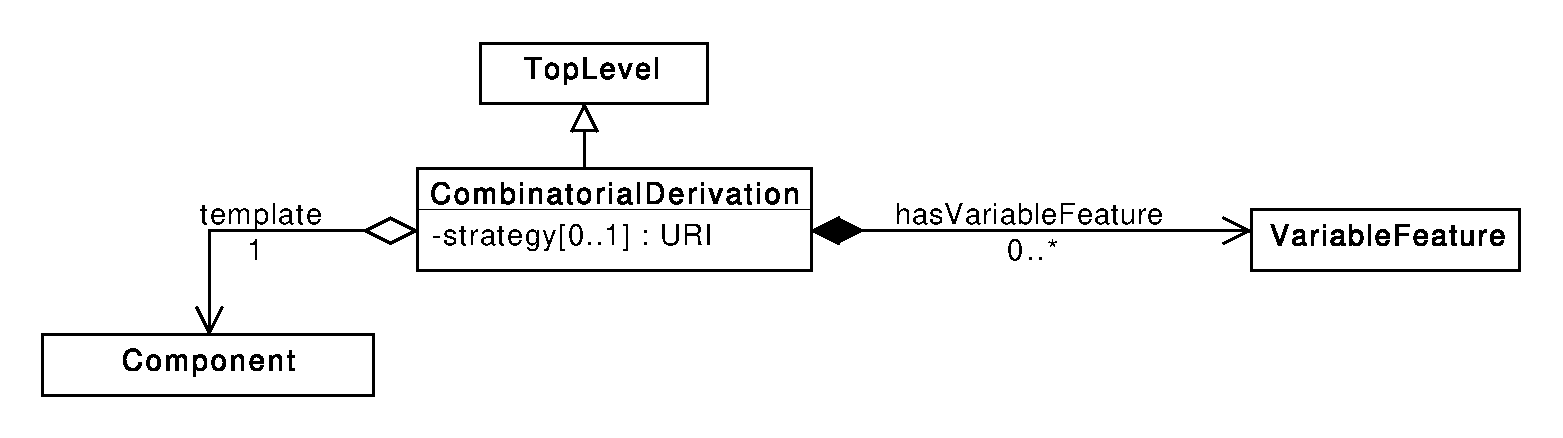
\includegraphics[scale=0.6]{uml/combinatorial_derivation}
\caption[]{Diagram of the \sbol{CombinatorialDerivation} class and its associated properties.}
\label{uml:combinatorial_derivation}
\end{center}
\end{figure}

\subparagraph{ The \sbolheading{template} property}\label{sec:template}

The \sbol{template} property is REQUIRED and MUST contain a URI that refers to a \sbol{Component}. 
This \sbol{Component} is expected to serve as a template for the derivation of new \sbol{Component} objects. 
Consequently, its \sbol{feature}s property SHOULD contain one or more \sbol{Feature} objects that describe its substructure (referred to hereafter as template \sbol{Feature} objects), and its \sbol{constraint} property MAY also contain one or more \sbol{Constraint} objects that constrain this substructure.

When a \sbol{Component} is derived in accordance with a \sbol{CombinatorialDerivation}, the \sbol{prov:wasDerivedFrom} property of the derived \sbol{Component} SHOULD refer to the \sbol{CombinatorialDerivation}. When multiple \sbol{Component} objects are derived in accordance with the same \sbol{CombinatorialDerivation}, they MAY be referred to by the \sbol{members} property of a \sbol{Collection}, in which case the \sbol{prov:wasDerivedFrom} property of the \sbol{Collection} SHOULD also refer to this \sbol{CombinatorialDerivation}.

If the \sbolmult{types:CD}{types} property of the template \sbol{Component} contains one or more URIs, then the \sbolmult{types:CD}{types} property of the derived \sbol{Component} SHOULD also contain those URIs. The same holds true for the \sbolmult{roles:CD}{roles} properties of these \sbol{Component} objects.

\subparagraph{ The \sbolheading{variableComponents} property}\label{sec:variableComponents}

The \sbol{variableComponents} property is OPTIONAL and MAY contain a set of \sbol{VariableComponent} objects. These \sbol{VariableComponent} objects are expected to denote the choices available when deriving the substructure of a new \sbol{Component} in accordance with a \sbol{CombinatorialDerivation}. The \sbol{variableComponents} property MUST NOT contain two or more \sbol{VariableComponent} objects that refer to the same template \sbol{Feature} via their \sbol{variable} properties.

If the \sbol{variable} property of one of these \sbol{VariableComponent} objects refers to a template \sbol{Feature}, then the \sbol{feature}s property of the derived \sbol{Component} SHOULD contain as many \sbol{Feature} objects derived from the template \sbol{Feature} as specified by the \sbol{operator} property of the \sbol{VariableComponent} (see \ref{tbl:operator}). In addition, the \sbol{instanceOf} properties of these derived \sbol{Feature} objects MUST refer to \sbol{Component} objects specified by the \sbol{variants}, \sbol{variantCollections}, or \sbol{variantDerivations} property of the \sbol{VariableComponent}.

If no \sbol{variable} property of one of these \sbol{VariableComponent} objects refers to a template \sbol{Feature}, then the \sbol{feature}s property of the derived \sbol{Component} SHOULD contain exactly one \sbol{Feature} with a \sbol{prov:wasDerivedFrom} property that refers to the template \sbol{Feature}. The \sbol{instanceOf} property of this derived \sbol{Feature} MUST refer to the \sbol{Component} referred to by the \sbol{instanceOf} property of the template \sbol{Feature}.

Finally, all of these derived \sbol{Feature} objects MUST follow the \sbol{restriction} properties of any \\
\sbol{Constraint} objects that refer to their corresponding template \sbol{Feature} objects.

\subparagraph{ The \sbolheading{strategy} property}\label{sec:strategy}
The \sbol{strategy} property is OPTIONAL and has a data type of URI. \ref{tbl:strategy} provides a list of REQUIRED \sbol{strategy} URIs. If the \sbol{strategy} property is not empty, then it MUST contain a URI from \ref{tbl:strategy}. This property recommends how many \sbol{Component} objects a user SHOULD derive from the template \sbol{Component}.


\begin{table}[ht]
  \begin{edtable}{tabular}{lp{4in}}
    \toprule
    \textbf{Strategy URI} & \textbf{Description} \\
    \midrule
    \url{http://sbols.org/v2#enumerate}  &  A user SHOULD derive all possible \sbol{Component} objects specified by the \sbol{CombinatorialDerivation}. \\
        \url{http://sbols.org/v2#sample}  & A user SHOULD derive a subset of all possible \sbol{Component} objects specified by \sbol{CombinatorialDerivation}. The manner in which this subset is chosen is for the user to decide. \\
    \bottomrule
  \end{edtable}
  \caption{REQUIRED \sbol{URI}s for the \sbol{strategy} property.}
  \label{tbl:strategy}
\end{table}


\subsubsection{VariableComponent}
\label{sec:VariableComponent}

The \sbol{VariableComponent} class can be used to specify a choice of \sbol{Component} objects for any new \sbol{SubComponent} derived from a template \sbol{SubComponent} in the template \sbol{Component}. This specification is made using the class properties \sbol{variable}, \sbol{variants}, \sbol{variantCollections}, and \sbol{variantDerivations} (see \ref{uml:variable_component}). While the \sbol{variants}, \sbol{variantCollections}, and \sbol{variantDerivations} properties are OPTIONAL, at least one of them MUST NOT be empty. If these properties contain duplicate URIs, then they SHOULD be treated as a single URI for the purpose of selection. For example, if the \sbol{variants} property contains two copies of URI $A$ and one copy of URI $B$, $A$ SHOULD NOT be selected twice during enumeration, and it SHOULD NOT be selected twice as much as $B$ during sampling.

\begin{figure}[ht]
\begin{center}
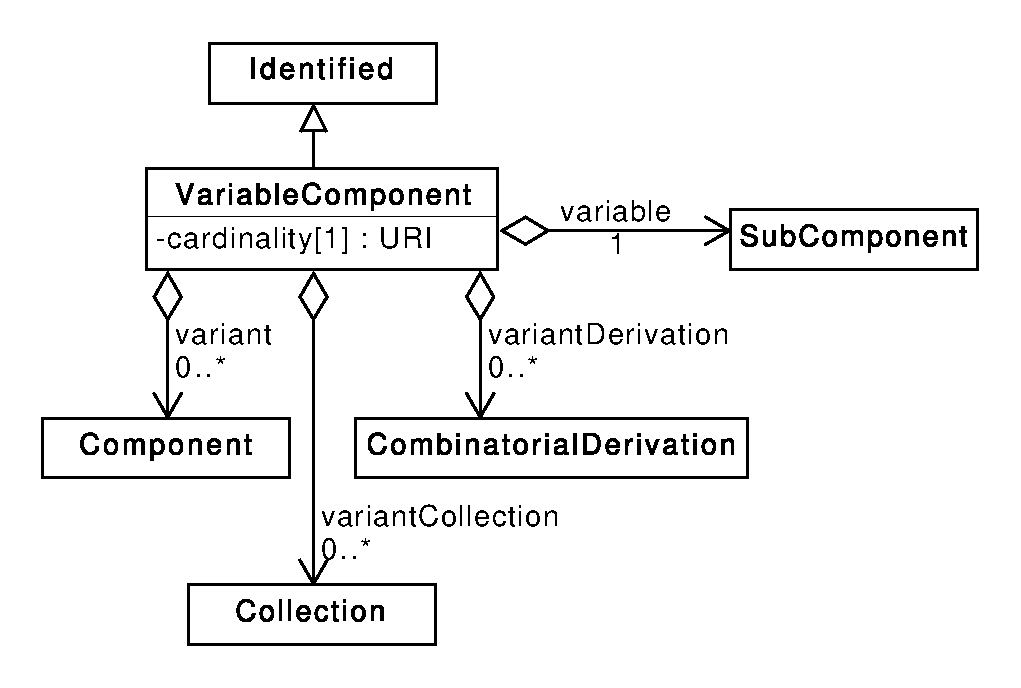
\includegraphics[scale=0.6]{uml/variable_component}
\caption[]{Diagram of the \sbol{VariableComponent} class and its associated properties.}
\label{uml:variable_component}
\end{center}
\end{figure}

\subparagraph{ The \sbolheading{variable} property}\label{sec:variable}

The \sbol{variable} property is REQUIRED and MUST contain a URI that refers to a template \sbol{SubComponent} in the template \sbol{Component}. If the \sbol{prov:wasDerivedFrom} property of a \sbol{SubComponent} refers to this template \sbol{SubComponent}, then the \sbol{instanceOf} property of the derived \sbol{SubComponent} MUST refer to either (1) a \sbol{Component} referred to by the \sbol{variants} property of the \sbol{VariableComponent}, (2) a \sbol{Component} from a \sbol{Collection} referred to by the \sbol{variantCollections} property of the \sbol{VariableComponent}, or (3) a \sbol{Component} derived from a \sbol{CombinatorialDerivation} referred to by the \sbol{variantDerivations} property of the \sbol{VariableComponent}.

If the \sbolmult{roles:CD}{roles} property of the template \sbol{SubComponent} contains one or more URIs, then the \sbolmult{roles:CD}{roles} property of the derived \sbol{SubComponent} SHOULD also contain those URIs.

\subparagraph{ The \sbolheading{variants} property}\label{sec:variants}

The \sbol{variants} property is OPTIONAL and MAY contain zero or more URIs that each refer to a \sbol{Component}. This property specifies individual \sbol{Component} objects to serve as options when deriving a new\\
\sbol{SubComponent} from the template \sbol{SubComponent}.

\subparagraph{ The \sbolheading{variantCollections} property}\label{sec:variantCollections}

The \sbol{variantCollections} property is OPTIONAL and MAY contain zero or more URIs that each refer to a\\
\sbol{Collection}. The \sbol{members} property of each \sbol{Collection} referred to in this way MUST NOT be empty. This property enables the convenient specification of existing groups of \sbol{Component} objects to serve as options when deriving a new \sbol{SubComponent} from the template \sbol{SubComponent}.

\subparagraph{ The \sbolheading{variantDerivations} property}\label{sec:variantDerivations}

The \sbol{variantDerivations} property is OPTIONAL and MAY contain zero or more URIs that each refer to a\\ \sbol{CombinatorialDerivation}. This property enables the convenient specification of \sbol{Component} objects derived in accordance with another \sbol{CombinatorialDerivation} to serve as options when deriving a new \sbol{SubComponent} from the template \sbol{SubComponent}. The \sbol{variantDerivations} property of a \sbol{VariableComponent} MUST NOT refer to the \sbol{CombinatorialDerivation} that contains this \sbol{VariableComponent}. Furthermore, \sbol{VariableComponent} objects MUST NOT form a cyclical chain of references via their \sbol{variantDerivations} properties and the\\ \sbol{CombinatorialDerivation} objects that contain them. For example, consider the \sbol{VariableComponent} objects A and B and the \sbol{CombinatorialDerivation} objects X and Y. The reference chain X contains A, A has variant derivation Y, Y contains B, and B has variant derivation X is cyclical.

\subparagraph{ The \sbolheading{operator} property}\label{sec:operator}

The \sbol{operator} property is REQUIRED and has a data type of URI. This property specifies how many \sbol{SubComponent} objects SHOULD be derived from the template \sbol{SubComponent} during the derivation of a new \sbol{Component}. The URI value of this property MUST come from the URIs provided in~\ref{tbl:operator}.


\begin{table}[ht]
  \begin{edtable}{tabular}{lp{4in}}
    \toprule
    \textbf{Operator URI} & \textbf{Description} \\
    \midrule
    \url{http://sbols.org/v2#zeroOrOne} & No more than one \sbol{SubComponent} in the derived \sbol{Component} SHOULD have a \sbol{prov:wasDerivedFrom} property that refers to the template \sbol{SubComponent}. \\
        \url{http://sbols.org/v2#one} & Exactly one \sbol{SubComponent} in the derived \sbol{Component} SHOULD have a \sbol{prov:wasDerivedFrom} property that refers to the template \sbol{SubComponent}. \\
\url{http://sbols.org/v2#zeroOrMore} & Any number of \sbol{SubComponent} objects in the derived \sbol{Component} MAY have \sbol{prov:wasDerivedFrom} properties that refer to the template \sbol{SubComponent}. \\
\url{http://sbols.org/v2#oneOrMore} & At least one \sbol{SubComponent} in the derived \sbol{Component} SHOULD have a \sbol{prov:wasDerivedFrom} property that refers to the template \sbol{SubComponent}. \\
    \bottomrule
  \end{edtable}
  \caption{REQUIRED \sbol{URI}s for the \sbol{operator} property.}
  \label{tbl:operator}
\end{table}

